\section{Privacy Preserving Histograms}\label{s:histograms}
Despite the challenges presented in sections \ref{s:challenges} and \ref{s:simple-algorithms}, the majority of algorithms can be transformed to their privacy preserving equivalent.
However, this is not a straightforward translation , as we examined in section \ref{s:simple-algorithms}, and in most cases it adds a complexity overhead to every algorithm that depends its control flow decisions in private data.

Histograms is a practical and notable example of algorithms that are widely used and the complexity of their privacy preserving version remains in computationally feasible levels, comparing to the textbook algorithm.
But first of all, what is a histogram?

As stated in \cite{ioannidis2003history}, histograms initially conceived as a visual aid to statistical approximations.
Webster’s defines a histogram as ``a bar graph of a frequency distribution in which the widths of the bars are proportional to the classes into which the variable has been divided and the heights of the bars are proportional to the class frequencies".
A histogram is generally a form of classifying and representing data in some categories of a specific range; the range is an individual ``base" element associated with each column.

More specifically, a histogram on some attributes $\{A, B, \dots, Z\}$ is constructed by partitioning the data distribution of those attributes into some ranges which are mutually disjoint subsets called buckets and approximating the frequencies and values in each bucket.
For the sake of simplicity let us suppose that the number of ranges ($\beta$) of all attributes are equal ($\beta \geq 1$).

In figure \ref{f:simple-hist} we present two histograms, the first one-dimensional over the attribute ``Patient Age" and the second is a two-dimensional over the attributes ``Patient Age" and ``Heart rate".
In both histograms $\beta = 4$, since the range of values for each attribute has been partitioned in four mutually disjoint subsets.
In the 1-dimensional histogram \ref{f:simple-hist}.a the $y-axis$ corresponds to the total number of occurrences of values that belong to each bucket.
In the 2-dimensional histogram \ref{f:simple-hist}.b since $y-axis$ corresponds to the ranges for the buckets for the second attribute, the occurrences are depicted with different colors.

\begin{figure}[t]
    \centering
    \subfloat[1D Numerical Histogram]{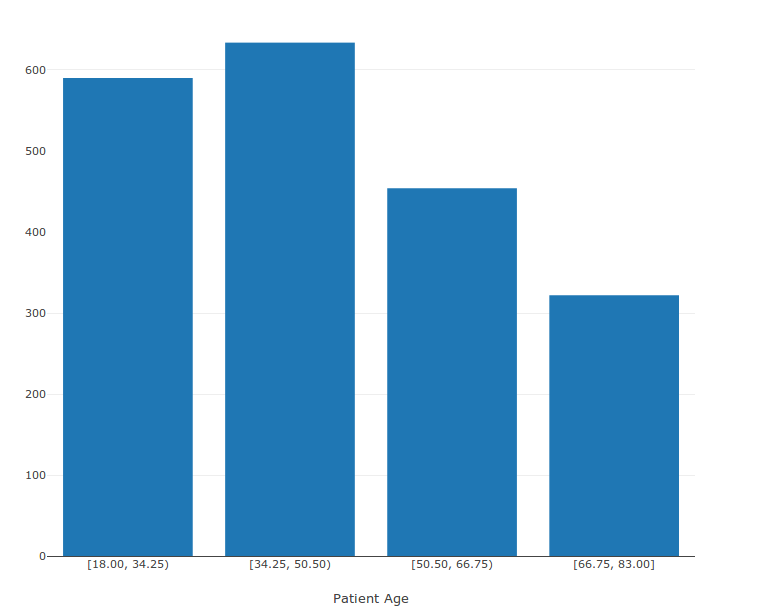
\includegraphics[width=0.49\columnwidth]{figures/1d-simple-hist.png}}
    \subfloat[2D Numerical Histogram / Heatmap]{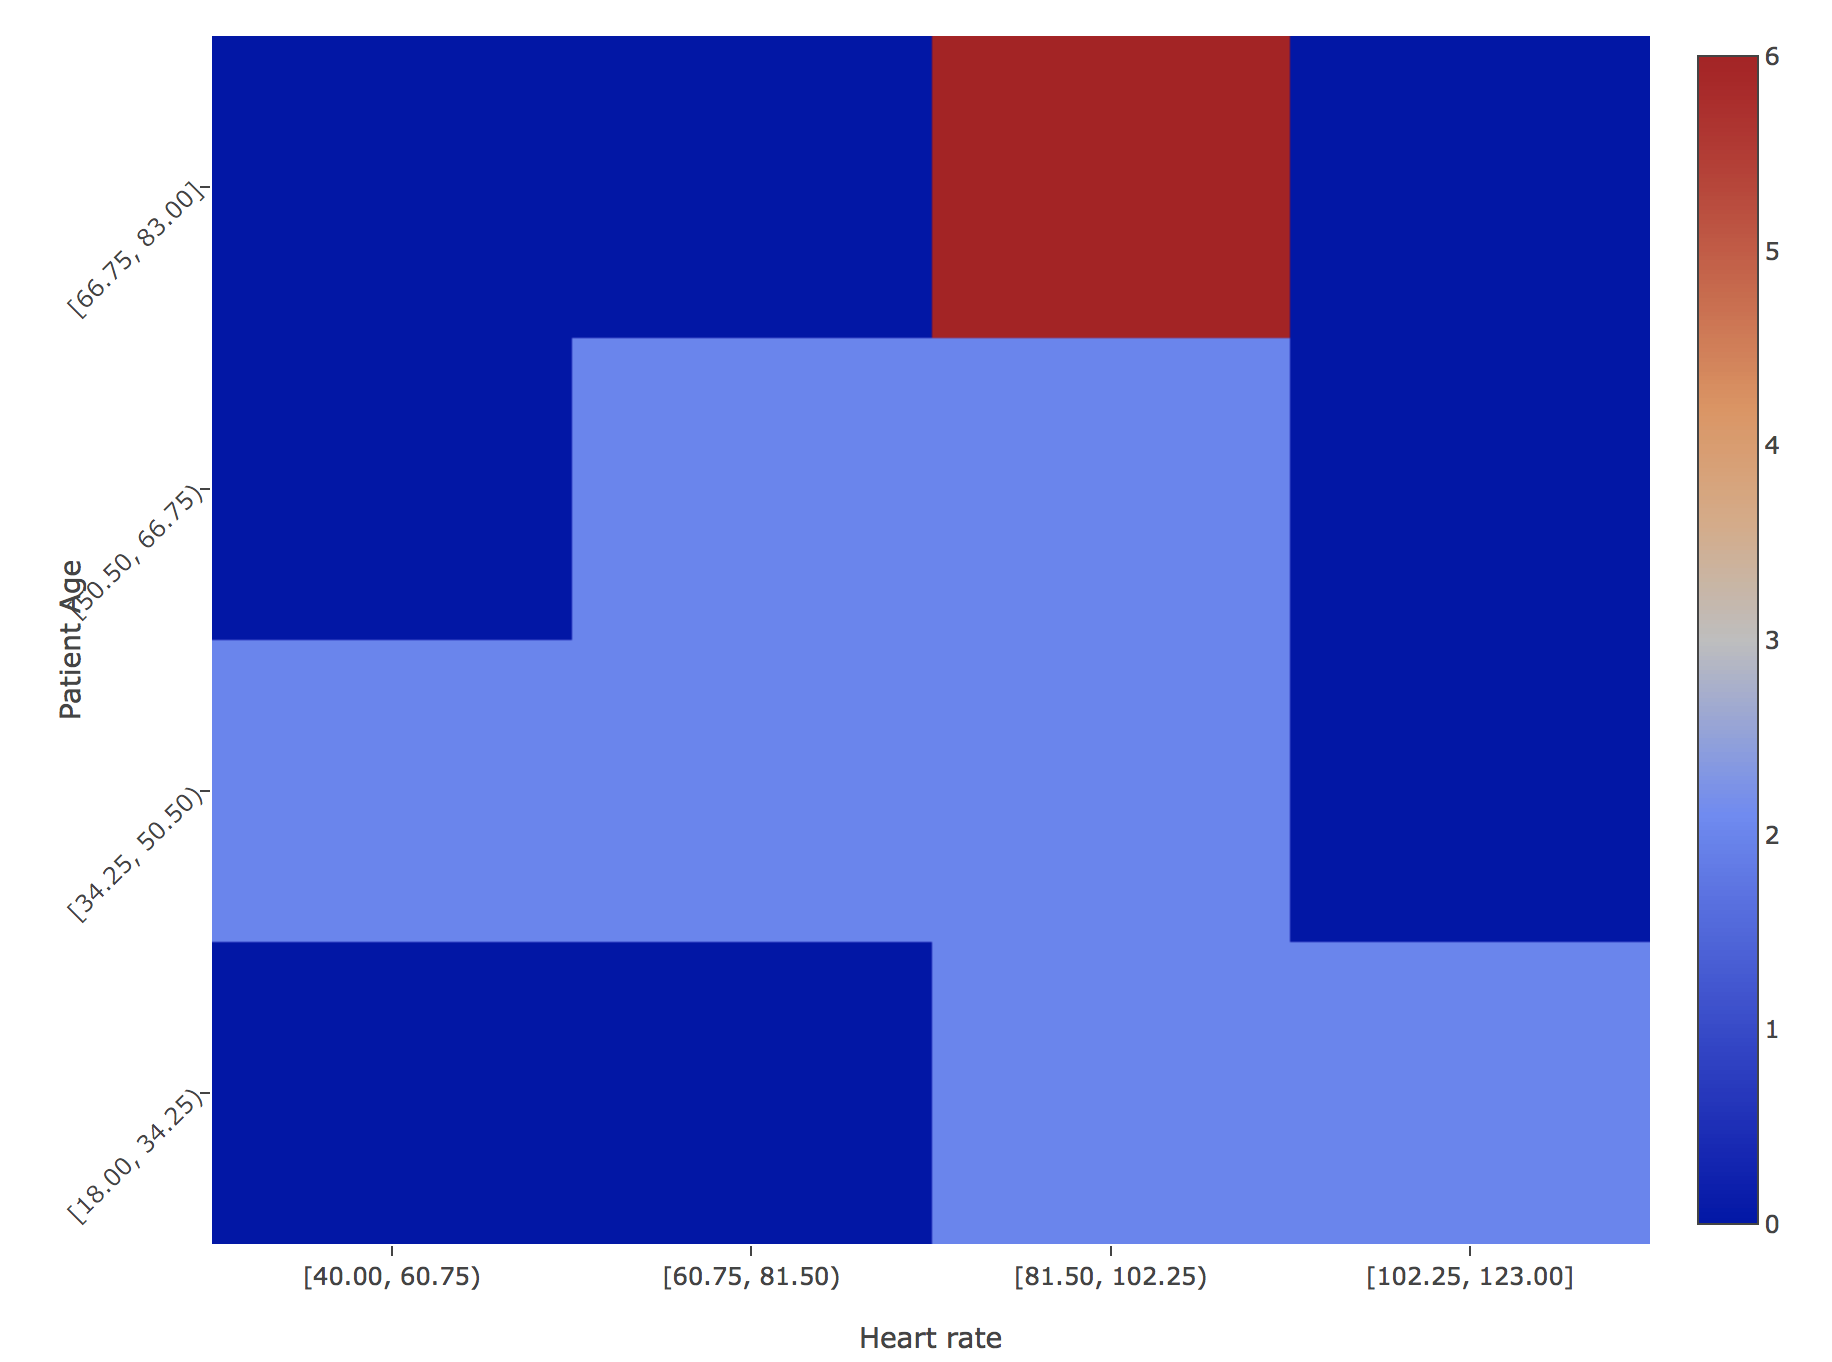
\includegraphics[width=0.49\columnwidth]{figures/2d-simple-hist.png}}

    \caption{(a) An one-dimensional histogram with $\beta = 4$,
    (b) A two-dimensional histogram with $\beta = 4$.}
    \label{f:simple-hist}
\end{figure}

\begin{figure}[t]
    \centering
    \subfloat[1D Categorical Histogram]{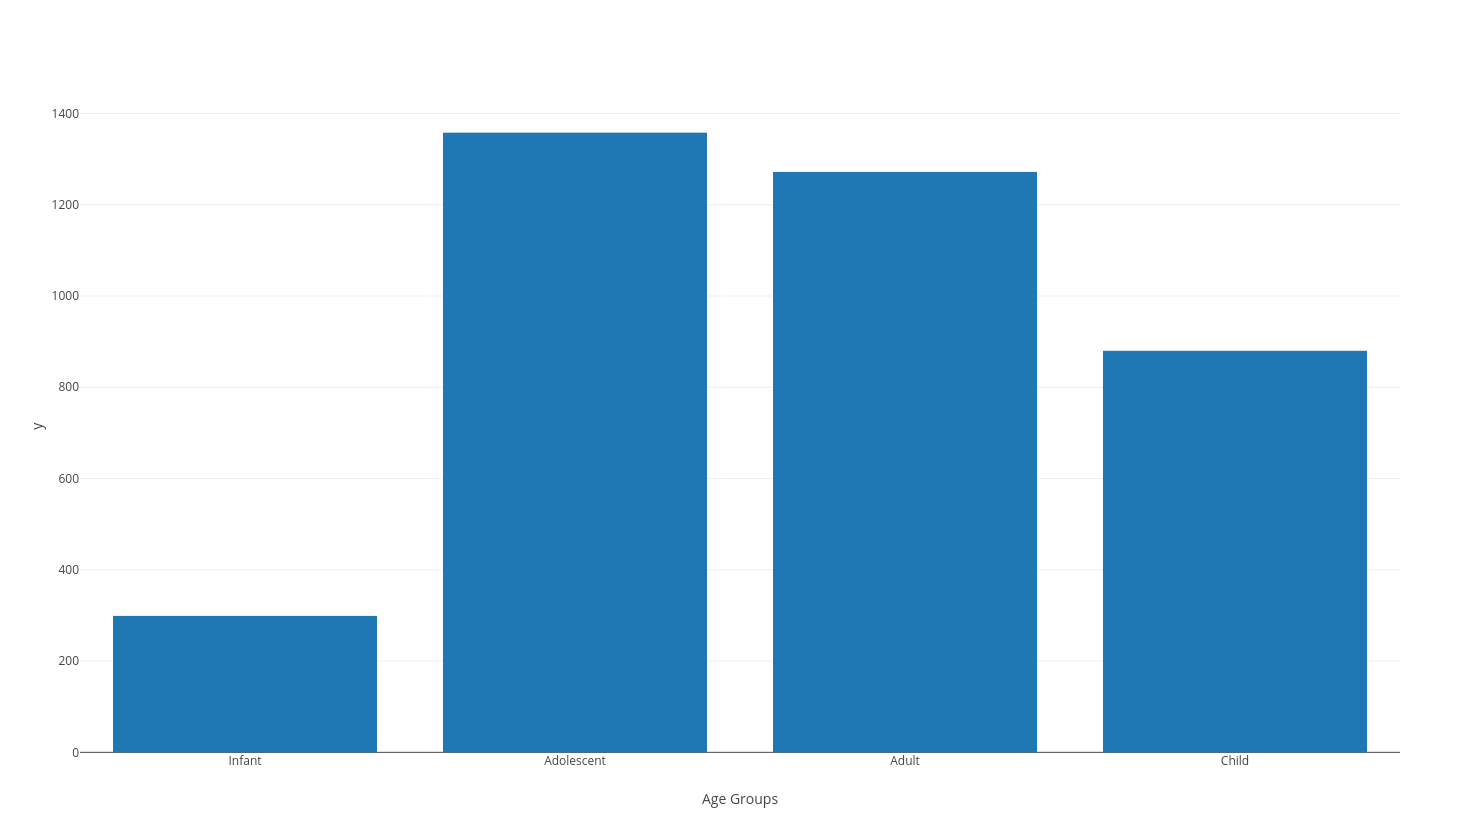
\includegraphics[width=0.49\columnwidth]{figures/AgeGroups.png}}
    \subfloat[2D Categorical Histogram / Heatmap]{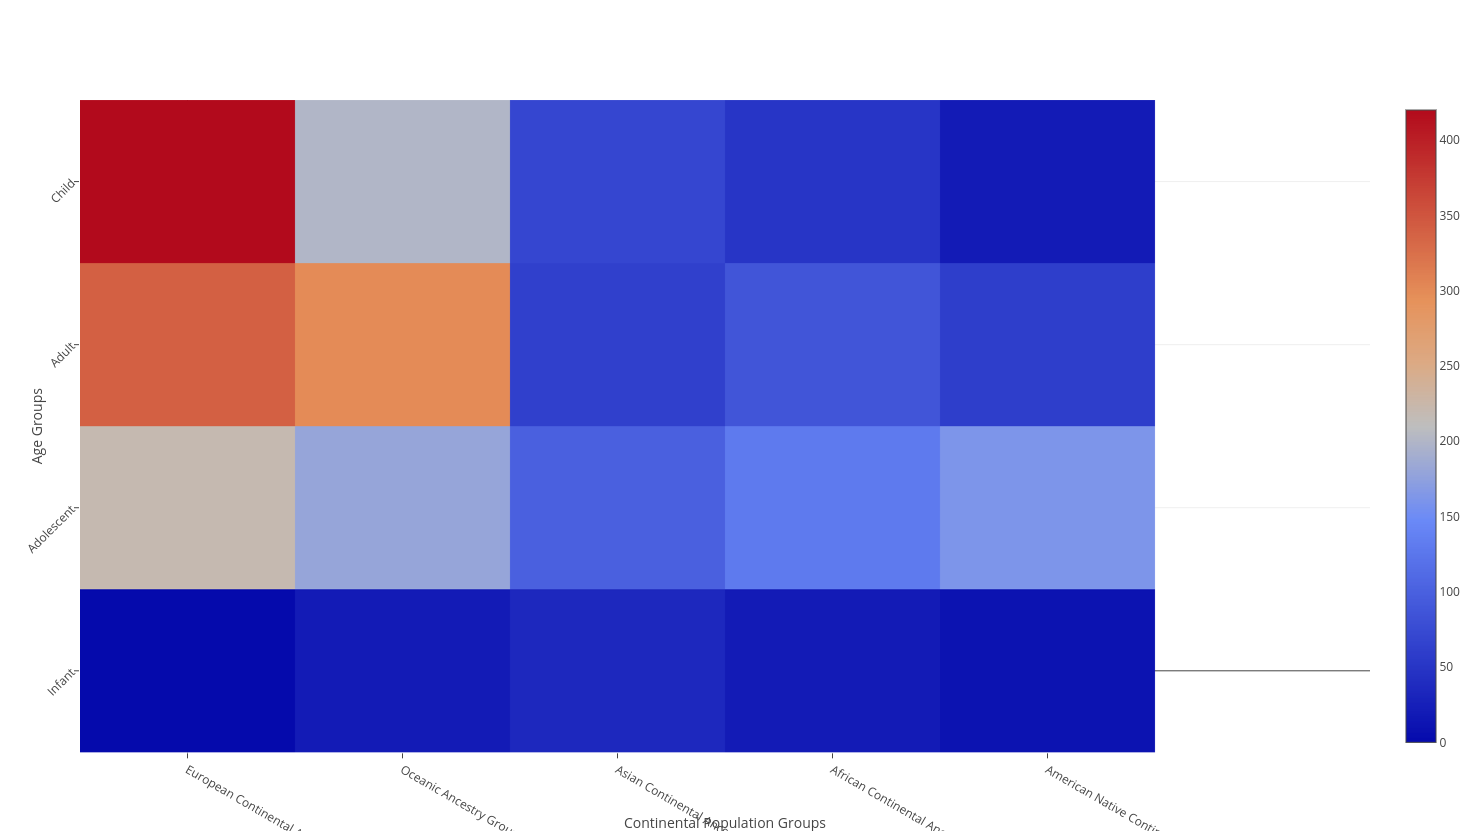
\includegraphics[width=0.49\columnwidth]{figures/AgeGroups_PopulationGroups.png}}

    \caption{(a) One-dimensional histogram displaying age groups,
    (b) A two-dimensional histogram displaying age groups with continental population groups.}
    \label{f:simple-categorical-hist}
\end{figure}

Similarly, in figure \ref{f:simple-categorical-hist} we present two more histograms, but with categorical values.
The attribute ``Age Groups" in \ref{f:simple-categorical-hist}.a is separated in four disjoint categories; ``Infant", ``Adolescent", ``Child" and ``Adult".
In \ref{f:simple-categorical-hist}.b we present demographic information (attribute ``Continental Population Groups") in relation with ``Age Groups".





\subsection{Algorithms for Privacy Preserving Histograms}\label{ss:histogram-algos}
Histograms are one of the simplest ways to visualize and easily understand data; rendering them very useful in many data analysis applications.
As we already mentioned, histograms consist of bars that are mutually disjoint and their heights are proportional to the counts of values in the corresponding ranges.

\textbf{Challenges with Privacy-Preserving Histograms}: The textbook algorithm splits the dataset to buckets and consecutively for each item it increments the corresponding ``bucket-counter".
Implementing this algorithm with respect to the privacy of the dataset introduces the problem that for each value it is not trivial to find the bucket that this specific value should be placed.

For instance, let us suppose that we are constructing the histogram in figure \ref{f:simple-hist}.a.
In this case $\beta = 4$, thus the algorithm should obliviously split the values into four disjoint buckets.
The range of each bucket is computed considering the $\beta$ parameter, as well as the minimum and maximum age in the dataset.
In this specific example, the minimum age is $18$, while the maximum is $83$.
Having $\beta = 4$ results to bucket-range $(83 - 18) / 4 = 16.25$.
Therefore, the ranges for attribute ``Patient Age" are formed as follows: $[18, 34.25), [34.25, 50.50), [50.50, 66.75), [66.75, 83]$.
Consecutively, for each patient in the dataset the algorithm calculates the number of bucket that the patient belongs by dividing his/her value with the bucket-range; however, this index is encrypted.
Finally, the algorithm iterates through all $\beta$ buckets and obliviously adding $\enc{1}$ if the bucket is the correct one, or $\enc{0}$ otherwise.

The aforementioned algorithm works for numerical values; however, the one for categorical values is very similar.
Bucket-range is fixed to one, and $\beta$ equals to all different possible values in the dataset.
Also, there is no notion of terms minimum and maximum in categorical values.


\subsubsection{Privacy Preserving Histogram Computation: A Naive Approach}\label{sss:histogram-simple}
As we mentioned in section \ref{s:two-types-of-data}, we have separated our algorithms in two major categories, for categorical and for numerical data.
The procedure described in \ref{ss:histogram-algos} is shown in algorithms \ref{a:1d-simple-histogram-categorical} and \ref{a:1d-simple-histogram-numerical}.
These algorithms iterate through all $N$ items and check all possible cells for that item.
When the correct cell is found, they increment the corresponding counter.
The former is tailored to categorical datasets, while the latter is tailored to numerical/continuous values.

\import{./}{algorithms/hist_simple_categorical.tex}

\import{./}{algorithms/hist_simple_numerical.tex}

Both algorithms are straightforward and simple to understand, however, not very efficient.
In the following subsections we delve into details for the privacy preserving algorithms that are based in the same idea, but leverage \texttt{SIMD} operations.


\subsubsection{Privacy Preserving Histograms for Categorical Values}\label{sss:histogram-categorical}
\textbf{One-Dimensional Histograms}: In algorithm \ref{a:1d-histogram-categorical} we present the privacy preserving algorithm of an one-dimensional (1D) histogram for categorical values.
In simple words, categorical data means that the values are discrete.
Hence, the second parameter in the algorithm (dubbed $P$) is the number of possible choices that exist in $array[N]$.
The input data is given in the form of a private array/vector.

The algorithm creates a boolean array of equal size as the input data, and then for each possible encrypted value of the dataset checks (line 3) and counts (line 4) its occurrences.
Method {\fontfamily{lmss} $\textsc{Sum}$} is the same as in algorithm \ref{a:sum}.
Finally, the counts are gathered into a vector and returned -- still encrypted -- to the user.

\import{./}{algorithms/1d_hist_categorical.tex}



\textbf{Multi-Dimensional Histograms}: In algorithm \ref{a:multidim-histogram-categorical} we present the privacy preserving algorithm of multi-dimensional histograms for categorical values.
As in algorithm \ref{a:1d-histogram-categorical}, here, the third parameter ($Ps$) is the number of possible choices that exist in $array$.
However, since here the input data is a private array with multiple dimensions $array[N][M]$, the possible values should express the possible values for each dimension.
Thus, it is an array of $A$ slots, where $A$ is the number of attributes.

Similarly to the 1D algorithm, the multi-dimensional one creates a boolean array of \fixme{explain the algorithm}

\import{./}{algorithms/multdim_hist_categorical.tex}


\textbf{Filtering the Histograms' Results}: In the preceding algorithms, the data

\fixme{Add filters explanation. Maybe code?}



\subsubsection{Privacy Preserving Histograms for Numerical Values}\label{sss:histogram-numerical}

\textbf{One-Dimensional Histograms}: In algorithm \ref{a:1d-histogram-numerical} we present the privacy preserving algorithm of one-dimensional (1D) histograms for numerical values.
In contrast with the categorical data, numerical data are not discrete, which means that the buckets in which the histogram will separate the dataset should be fixed (the $\beta$ parameter, as mentioned in section \ref{s:histograms})

First and foremost, the input data is given in the form of a private array/vector of $N$ positions.
The second parameter is open (since the final results will eventually disclose it), and is the number of buckets/cells that the algorithm will create, namely the $\beta$ factor.
The two last parameters are also encrypted and are the minimum and maximum values found in the dataset/array (first parameter of the algorithm).
Those two parameters are necessary in order to determine for each element in the array in which cell should be placed.

This algorithm is very similar and in accord with algorithm \ref{a:1d-histogram-categorical}, however does some extra steps.
In lines 2 and 3, it first determines the width for each cell and then creates an array of $N$ elements that each one indicates the bucket that the element in the corresponding position of $array$ should be placed.
Consecutively, the algorithm creates another boolean array of equal size as the input data, and then for each possible encrypted value of the $cellMap$ checks (line 5) and counts (line 6) its occurrences.
Finally, the counts are gathered into a vector and returned -- still encrypted -- to the user.
Line 5 of algorithm \ref{a:1d-histogram-numerical} is more complex than line 3 of algorithm \ref{a:1d-histogram-categorical}, since the former has to check some corner cases of data that belong to the last bucket.

\import{./}{algorithms/1d_hist_numerical.tex}



\textbf{Multi-Dimensional Histograms}:
\fixme{probably move most of them in the numerical multidimensional since it appears first...}
The algorithm that computes a private multi-dimensional histogram is similar to the one regarding one-dimensional histograms but also addresses the issue of having a histogram of arbitrarily many dimensions.
In case we had a known number of dimensions the simplest solution would be to use nested loops, as many as the histogram dimensions.
Since the number of dimensions is not known, we have to think of something else.
We represent the multi-dimensional histogram as a serialized version with an one-dimensional array (a vector) instead of using a multi-dimensional array (a matrix).
For example a 2-dimensional $3 \times 4$ histogram will be represented as a vector whose length is $ 12 $ ($= 3 \cdot 4$), and a $3 \times 4 \times 5$ 3-dimensional histogram wit a vector of length $ 60 $ ($= 3 \cdot 4 \cdot 5$)

When it comes to indexing if we wish to access the 2-dimensional $N \times M$ histogram represented as an one-dimensional at row $ i $ and column $ j $, instead of using $h[i][j]$ we use $h[i \cdot M + j]$.
Similarly, for the 3-dimensional $L \times N \times M$ histogram, $h[i][j][k]$ becomes $h[i \cdot N \cdot M + j \cdot M + k]$. So there needs to be a computation of a single index based on the multiple dimension indexes. In algorithm \ref{a:multidim-histogram-numerical}, the \texttt{positions} vector holds this index for each record of the provided array, as can bee seen in lines $ 12 $ and $ 13 $

\import{./}{algorithms/multdim_hist_numerical.tex}


Filters here are easily applied as in \ref{sss:histogram-categorical} ... \fixme{some exaplanation ..}


